\subsection{Bilanzierung}

%%%%%%%%%%%%%%%%%%%%%%%%%%%%%%%%%%%%%%%%%%%%%%%%%%%%%%%%%%%%%%%%%%%%%%%%%%%%%%%%%%%%%%%%%%%%%%%%%%%%%%%%%%%%%%%%%%%%%%%%%%%%%%%%%%%%%%%%%%%%%%%%%%%%%%%%%%%%%%%%%%%
\subsubsection{Kontext der Bilanzierung}

Bilanzierung ist ein Konzept welches in unterschiedlichen Einsatzbereichen verwendung findet. Diese Forschung befasst sich mit Bilanzräumen 
im Kontext der DIN EN ISO 50001:2018-12. Die Norm setzt den Schwerpunkt auf die fortlaufende Verbesserung der energiebezogenen Leistung 
(\cite[Kapitel 0.2]{DIN50001.2018}). Aufgrund dessen sollte die Bilanzierung in diesem Forschungskontext aus einer Perspektive betrachtet werden welche 
energiebezogene Größen betrachtet.

Auch die Festlegung auf Organisationen des tertiären Wirtschaftssektors hat auswirkungen auf die betrachtungsweise der Bilanzierung. 
Denn in Organisation mit immateriellen Dienstleistungen spielt die Gebäudeenergie eine vorrangige Rolle zur Verbesserung der energiebezogenen 
Leistung (\cite[S. 3]{Fichera.2020}). 
Dies lässt sich Beispielhaft an der Abbildung \eqref{fig:Energieverbrauch_Wärme_DE} darstellen.

\begin{figure}[H]
    \centering
    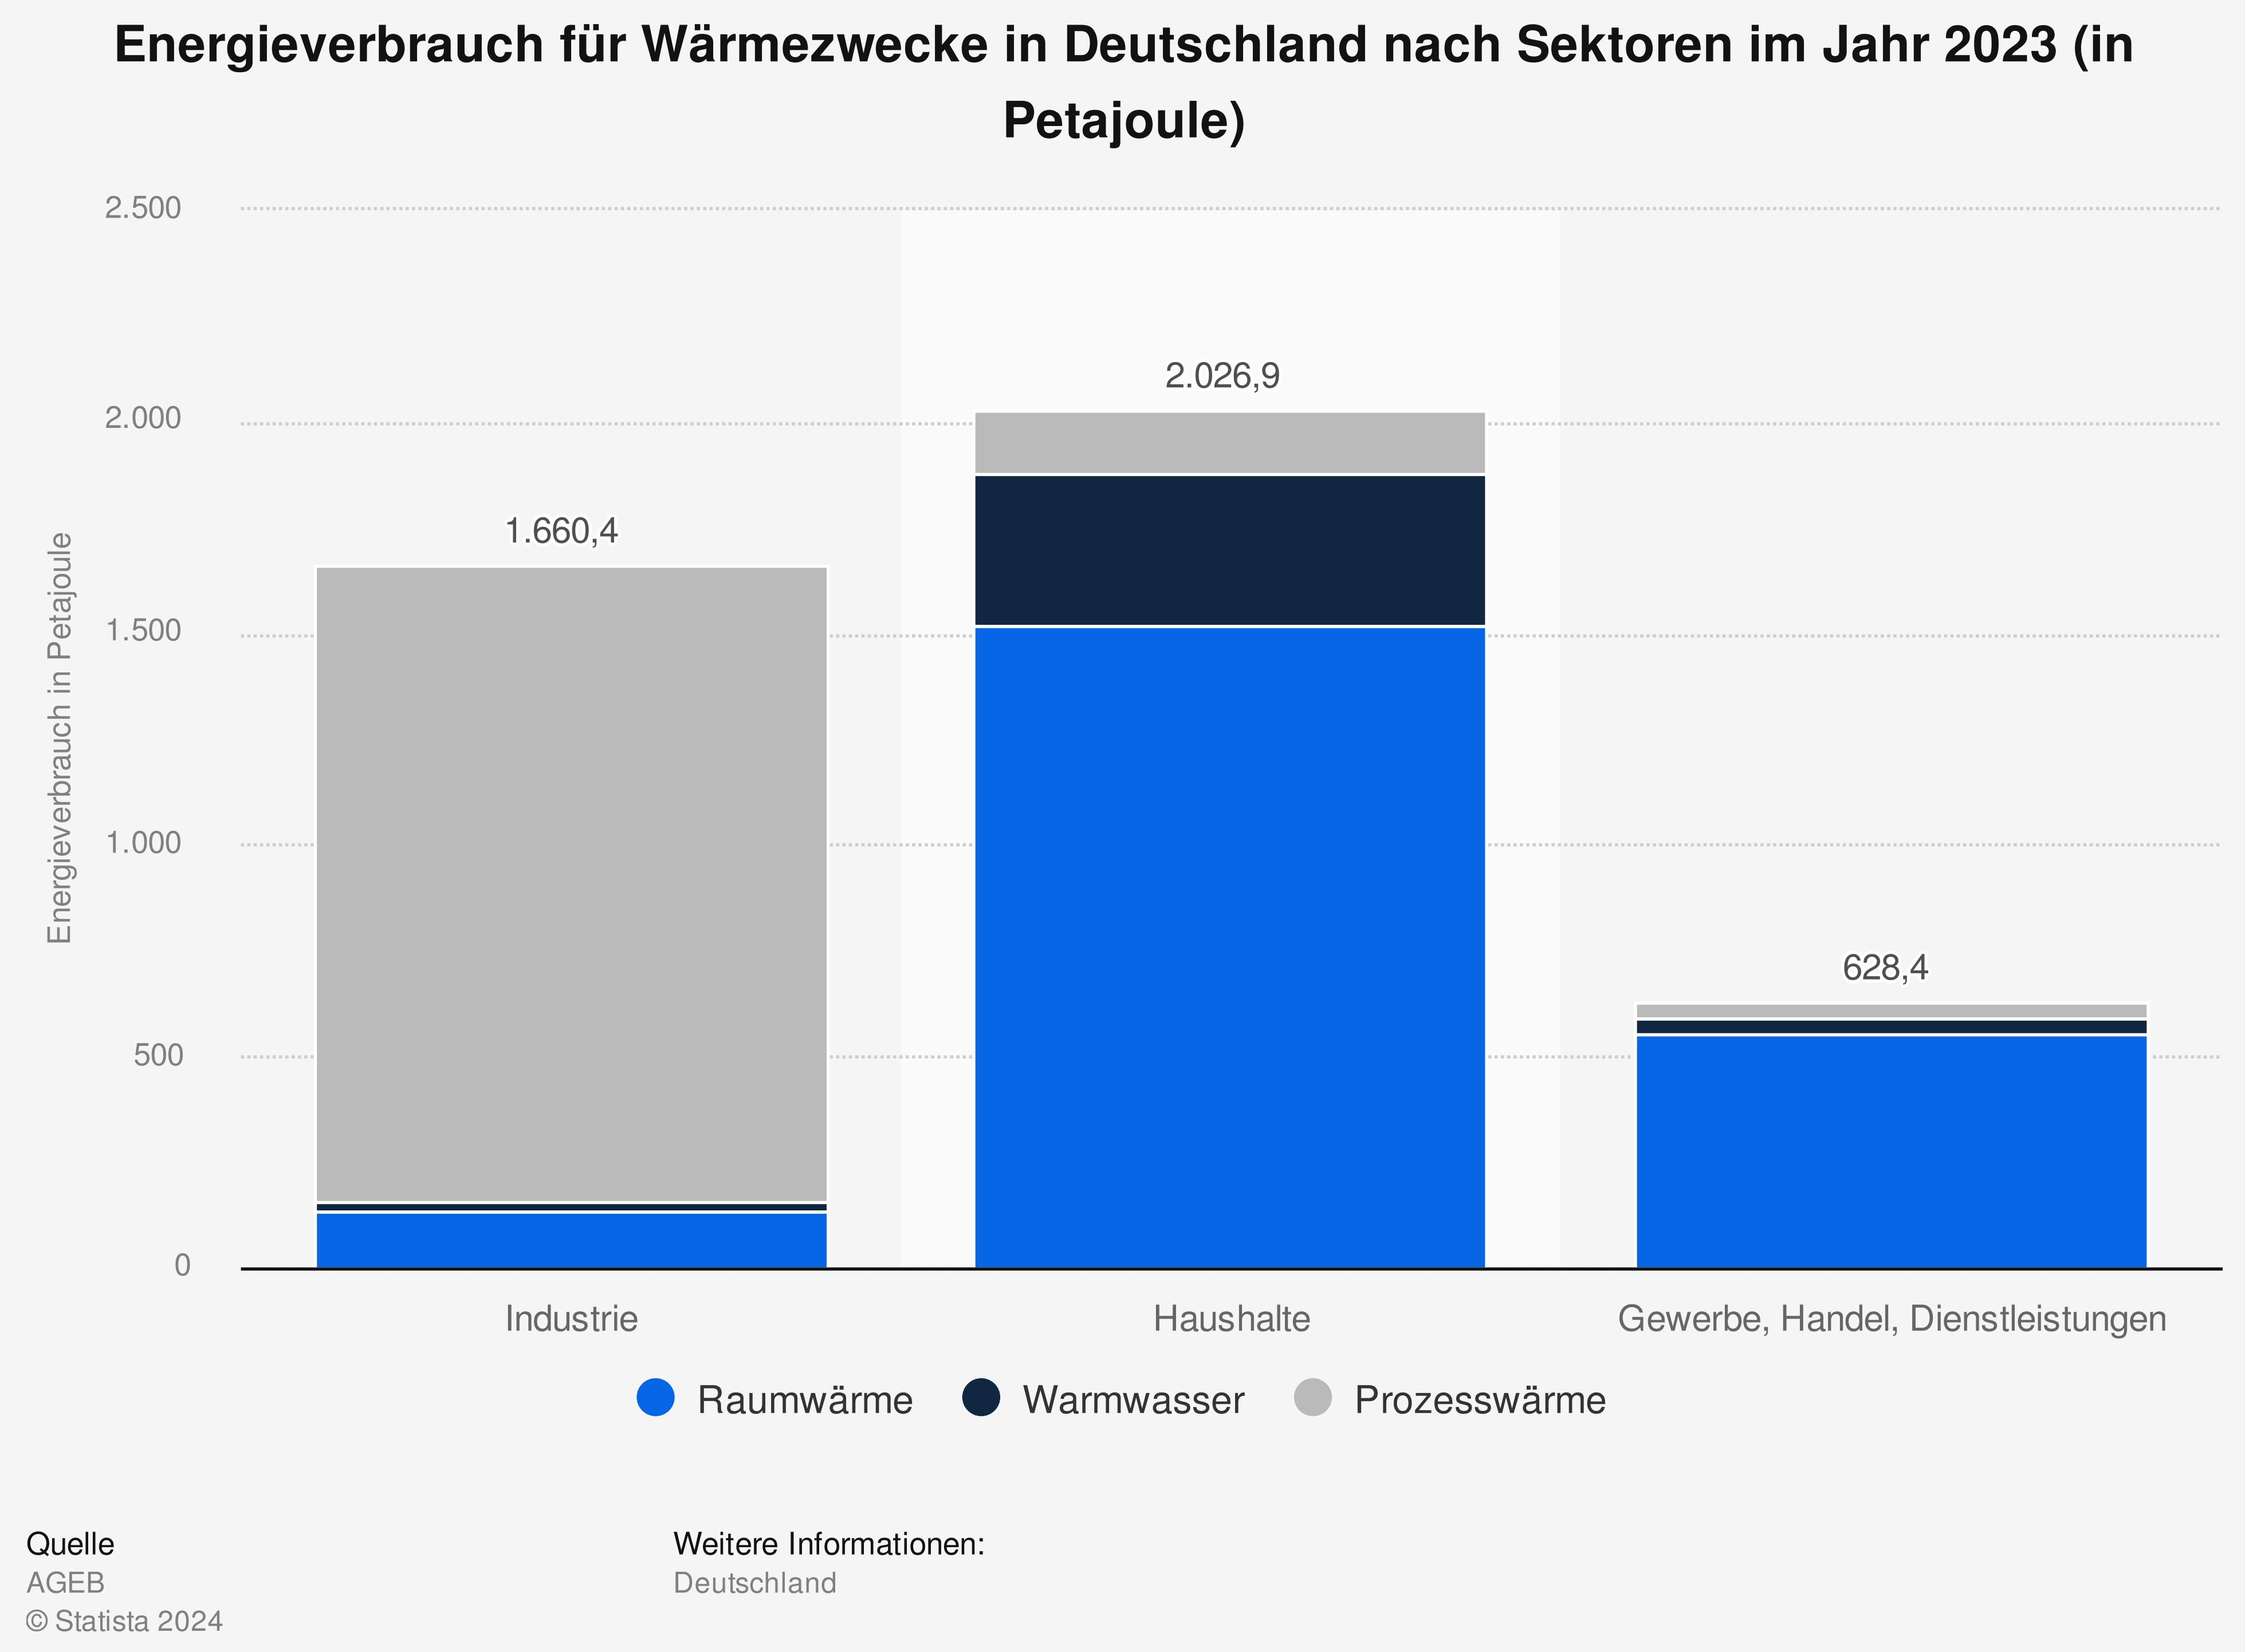
\includegraphics[width=0.68\textwidth]{../../Ressourcen/Bilder/Energieverbrauch_für_Wärmezweck_DE.jpg}
    \caption{Energieverbrauch für den Wärmezweck in Deutschland [\cite{AGEB.2024}]}
    \label{fig:Energieverbrauch_Wärme_DE}
\end{figure}

Die Abbildung \ref{fig:Energieverbrauch_Wärme_DE} zeigt den Energieverbrauch für Wärmezwecke in Deutschland im Jahr 2023, aufgeschlüsselt nach Sektoren. 
Während der industrielle Sektor einen hohen Anteil an prozessbezogener Wärme aufweist, spielt im Dienstleistungssektor die Raumwärme 
eine dominante Rolle.
Diese Statistik bekräftigt die Aussage von Fichera (2020, S. 3) dass bei der Verbesserung der energiebezogenen Leistung in Organisationen des tertiären 
Wirtschaftssektors energiebezogene Prozesse und Technologien im Gegensatz zur Gebäudeenergie eine untergeordnete Bedeutung haben. 

Im Rahmen der Bestimmung des Gesamtenergiebedarfs eines Gebäudes über den Lebenszyklus wird vor allem der Gebäudebetrieb betrachtet (\cite[S. 133]{Musall.2015}).
Die sogenannte Graue Energie wird üblicherweise als kumulierter, nicht erneuerbarer Primärenergieaufwand beschrieben, der alle vor- und nachgelagerten 
Prozesse der verwendeten Baustoffe und Materialien sowie der technischen Anlagen umfasst (\cite[S. 133]{Musall.2015}). Da die DIN EN ISO 50001:2018-12 
auf die fortlaufende Verbesserung der energiebezogenen Leistung abzielt und die Graue Energie konstant ist wird diese im Rahmen dieser Arbeit nicht 
betrachtet. 
Stattdessen liegt der Fokus dieser Forschungsarbeit auf der Bilanzierung energetischer Größen im Rahmen von Organisation des tertiäten Wirtschaftssektors. 
Sie grenzt sich somit von der Bilanzierung von Rohstoffen und Materialien ab.

%%%%%%%%%%%%%%%%%%%%%%%%%%%%%%%%%%%%%%%%%%%%%%%%%%%%%%%%%%%%%%%%%%%%%%%%%%%%%%%%%%%%%%%%%%%%%%%%%%%%%%%%%%%%%%%%%%%%%%%%%%%%%%%%%%%%%%%%%%%%%%%%%%%%%%%%%%%%%%%%%%%

\subsubsection{Definition Bilanzierung}
Im Rahmen des beschrieben Kontexts rückt die verfahrenstechnische Perspektive der Bilanzierung in den Fokus. 
So wird die Bilanzierung im Kontext der Verfahrenstechnik nach Rönsch (2015, S. 66) in drei Bilanzgleichungen unterteilt: 
die Massenbilanz, die Energiebilanz und die Impulsbilanz. 
Zur Beantwortung dieser Forschungsfrage hat insbesondere die Energiebilanz eine hohe Relevanz.

Die Energiebilanz beruht auf dem Energieerhaltungssatz (\cite[S. 66]{Rönsch.2015}), der das Prinzip der Erhaltung 
der Energie ausdrückt (\cite[S. 57]{Baehr.1966}). Der Energieerhaltungssatz bezieht sich auf alle Erscheinungsformen, in denen Energie auftritt, 
und besagt, dass es unmöglich ist, Energie zu erzeugen oder zu vernichten (\cite[S. 57]{Baehr.1966}). 
Für zu bilanzierende Systeme bedeutet dies, dass die Energie in einem abgeschlossenen, adiabaten System über die Zeit 
konstant ist (\cite[S. 66]{Rönsch.2015}). 
Adiabat bedeutet in diesem Kontext, dass das System keine Wärme mit seiner Umgebung austauscht (\cite[S. 66]{Rönsch.2015}). 

Für Systeme, die in der Lage sind, Energie zu speichern, impliziert dies nach Rönsch (2015, S. 66f.), 
dass die darin gespeicherte Energie gleich der Differenz aus ein- und austretenden Energieströmen ist. 
Für offene, nicht-adiabate Systeme ohne Speicherfähigkeit gilt, dass die Differenz der ein- und austretenden Energieströme Null ist 
(\cite[S. 66f.]{Rönsch.2015}).
Das von Rönsch (2015, S. 66f.) beschriebene Verhalten eines Systems bezüglich der Energiespeicherung, lässt sich mathematisch 
vereinfacht mit der Gleichung \eqref{energiebilanzierungsgleichung_Rönsch} darstellen:

\begin{equation}
E_{\text{gespeichert}} = \sum E_{\text{eingang}} - \sum E_{\text{ausgang}}
\label{energiebilanzierungsgleichung_Rönsch}
\end{equation}

\begin{description}
    \item \(E_{\text{gespeichert}}\): Im System gespeicherte Energie.
    \item \(E_{\text{eingang}}\): Energie eines eintretenden Energiestroms.
    \item \(E_{\text{ausgang}}\): Energie eines austretenden Energiestroms.
    \item Für offene, nicht-adiabate Systeme ohne Energiespeicher gilt:
    \[
    E_{\text{gespeichert}} = 0
    \]
    \item In diesem Fall ist die zugeführte Energie gleich der abgegebenen Energie:
    \[
    \sum E_{\text{eingang}} = \sum E_{\text{ausgang}}
    \]
\end{description}

Diese Gleichung beschreibt einen allgemeinen Ansatz zur Energiebilanzierung der im System gespeicherten Energie. 
Im Rahmen der Bilanzierung komplexer Systeme kann jedoch eine detailliertere Bilanzierung einzelner Zustandsgrößen im System erforderlich sein.

Dieses Problem wird von der von Ahrendts (2014, Kapitel 1.5) aufgestellten Bilanzgleichung im Kontext der Thermodynamik addressiert. 
Die Gleichung basiert auf dem Fakt, dass sich für jede mengenartige Zustandsgröße, die über die Grenze eines Systems transportiert wird, eine 
Bilanz aufstellen lässt (\cite[Kapitel 1.5]{Ahrendts.2014}). 
Diese Bilanz umfasst ein- und austretende Ströme sowie im System enthaltene Energiequellen und -senken und ermittelt die 
Geschwindigkeit der Änderung des Bestands der zu bilanzierenden Zustandsgröße im System (\cite[Kapitel 1.5]{Ahrendts.2014}).

Die von Ahrendts (2014, Kapitel 1.5) aufgestellte Bilanzgleichung wird in den Formeln \eqref{BilanzierungsgleichungAhrendt} und 
\eqref{BilanzierungsgleichungAhrendtStrom} dargestellt.

\begin{equation}
    dX_{\text{j}}/d\tau = (\sum \dot{X}_{\text{j,e}} - \sum \dot{X}_{\text{j,a}}) + (\dot{X}_{\text{j,Quell}} - \dot{X}_{\text{j,Senk}})
    \label{BilanzierungsgleichungAhrendt}
\end{equation}

\begin{description}
    \item \(X_{\text{j}}\): Zustandsgröße.
    \item \(\tau\): Zeitintervall.
    \item \(X_{\text{j,e}}\): Über die Systemgrenze zufließende Zustandsgröße.
    \item \(X_{\text{j,a}}\): Über die Systemgrenze abfließende Zustandsgröße.
    \item \(X_{\text{j,Quell}}\): Quellen der Zustandsgröße im System.
    \item \(X_{\text{j,Senk}}\): Senken der Zustandsgröße im System.
\end{description}

Im Rahmen der Formel \eqref{BilanzierungsgleichungAhrendt} wird der Strom einer Zustandsgröße \(X_{\text{j}}\) in Gleichung 
\eqref{BilanzierungsgleichungAhrendtStrom} definiert.

\begin{equation}
    \dot{X}_{\text{j}} = \lim_{\Delta\tau \to 0} \Delta X_{\text{j}}/ \Delta\tau
    \label{BilanzierungsgleichungAhrendtStrom}
\end{equation}

\begin{description}
    \item \(X_{\text{j}}\): Zustandsgröße.
    \item \(\Delta X_{\text{j}}\): Menge der Größe \(X_{\text{j}}\) im Zeitintervall \(\Delta \tau\).
    \item \(\Delta \tau\): Zeitintervall.
\end{description}

Die Gleichung \eqref{BilanzierungsgleichungAhrendt} in Verbindung mit \eqref{BilanzierungsgleichungAhrendtStrom} beschreibt die Geschwindigkeit 
der Änderung des Bestands der Größe \(X_{\text{j}}\) als Summe der Differenzen zwischen den über die Systemgrenze zu- und abfließenden Strömen der 
Zustandsgröße \(X_{\text{j}}\) sowie den Quell- und Senkströmen der Zustandsgröße \(X_{\text{j}}\) innerhalb des Systems.  
Somit formulieren die Gleichungen \eqref{energiebilanzierungsgleichung_Rönsch} und \eqref{BilanzierungsgleichungAhrendt} in Verbindung mit 
\eqref{BilanzierungsgleichungAhrendtStrom} eine grundlegende und zugleich vereinfachte mathematische Beschreibung einer Bilanzierung im Kontext 
der Thermodynamik und Verfahrenstechnik. Sie bilden die Basis für die Beschreibung der grundlegenden Struktur einer Bilanz.
Im Folgenden werden die in \eqref{energiebilanzierungsgleichung_Rönsch} und \eqref{BilanzierungsgleichungAhrendt} mit \eqref{BilanzierungsgleichungAhrendtStrom} 
beschriebenen Bestandteile einer Bilanz zur Konzeption eines Bilanzraums im Anwendungskontext des Problemraums analysiert. 

